\documentclass[a4paper,12pt]{article}

\usepackage{url, hyperref, graphicx}

\begin{document}

\title{Project 1 Checkpoint}
\author{Chip Bell}
\date{February 6th, 2015}
\maketitle

\section{Problem Description}
Traffic simulation is becoming increasing important due to the expansion and growth of cities. Long-standing
infrastructure is forced to adapt in order to accomodate greater amounts of traffic, despite the fact that in many
cases the roads cannot be modified. This can be a result of legislation, existing buildings, and private property among
other things. So as a result, cities must instead optimize the variables they can control. In this case, we consider
signal light timing for the 12th St. and Peachtree Street intersection. In particular,
we explore the effects that light timing has on traffic flow, given a source input distribution of cars.

\section{The Conceptual Model}
In order to create a representative software simulation of the aforementioned system, we first begin by designing a
conceptual version of this model from which we can plan our implementation. We'll borrow heavily from the results and data
in \cite{cts12} when formulating our model.
Our architecture will be event driven, prioritizing events by timestamp. Furthermore,
we'll utilize the publisher-subscriber pattern (see \cite{pubsub}) to promote better decoupling.
Given this architecture, our first step will be to identify the entities present in our model, and then consider their
interactions (or the inherent ``activies'') within the simulation. This will allow us then to design the events that
are important

\subsection{Entities}
The first entity, unsurprisingly, is a single car. Our representation of a car is clearly less detailed than the real
thing, but rather focuses on variables that influence it's travel time from its starting location to destination, along
with the variables that influence neighboring cars. For our simulation, we'll track the position and destination of the
cars, along with the size of the car since that can influence the position of cars behind it. Also, we will track the
current velocity of the car 

Another entity to consider is the intersection itself. It's changing in time constantly, and those changes affect
every entity within the simulation. The most important parameters to consider here are the light timings. This
intersection's timings are time-based, rather than sensor-based, which can be seen in the data set provided with the
project description and is also available online \cite{ngsim}. We assume that the current light timing provided here
are optimal, but because we'll have a computer simulation in the end we have free reign in experimenting with these
values and observing the outcome. Perhaps the timings are \emph{not} optimal. Perhaps, our model grossly oversimplifies
some crucial interaction within the system. This is perhaps the most exciting part of the project.

\subsection{Basic Interactions}
From the intersection entity, we can glean an important interaction that occurs: The changing of light signal. When a
signal changes, each car in-queue will be forced to change it's state, whether it's waiting or currently in motion.
From an event-driven perspective, this means that any listener would need to be able to know \emph{how} the light
changed in order to act accordingly.

An intersection serves as holding point for cars traveling along the road so if a light is red, cars are forced to
queue up at the intersection until green. This lends itself to a queue-style data structure that encorporates both
position and acceleration. Car acceleration is a complex topic, but models have been constructed \cite{bonneson}
\cite{herman_et_al}. These models are generally continuous, and can generally be represented as a differential equation
due to the relationships between acceleration and velocity, as can be seen in \cite{briggs} \cite{deceleration} as well.
Instead, we will
simply consider the various events that trigger changes in behavior. For instance, if a car slows down, the car behind
it will be notified and change it's driving patterns accordingly.

\subsection{Events}
Based on our observations from above, we can now construct a set of events that are pertinent to this application.

First off, signal changes consititute the major event in the system. When a signal changes, the event must contain
\emph{when} the signal changed, and \emph{what} the signal changed to. The light itself will listen for this event
and will enqueue the next signal change based on the signal change time. These signal changes could be enqueued
completely upfront, but allowing this to be done on the fly allows the user to tweak these values during the simulation.

The car model will listen for this event as well. When a currently traveling car sees a red light, it will calculate
\emph{where} it needs to stop, and \emph{when} it will come to a stop. This will be done using a deceleration model
similar to \cite{deceleration}. If the light turns to green, the car instead needs to start accelerating (using one of
the models mentioned above). The model will adapt to light changes during movement by recalculating its estimated
exit time of the system.

\subsection{Simulation Input}
The two main sources of input into this simulation are the cars entering out section of Peachtree St, and the light
timing of the system. The combination of these two variables are what influence the smoothness
of traffic flow to the actual drivers in the system.

We first concern ourselves with finding an input distribution for cars entering the system. In our model, we'll only
consider basic aspects of a car: when it enters the system, and it's intended destination (turning left or right at
12th street or going straight). We will assume that all cars have the same speed entering the system, and that they
have the same length. These values can be calculated from the NGSIM data set \cite{ngsim}.

\begin{figure}
\begin{center}  
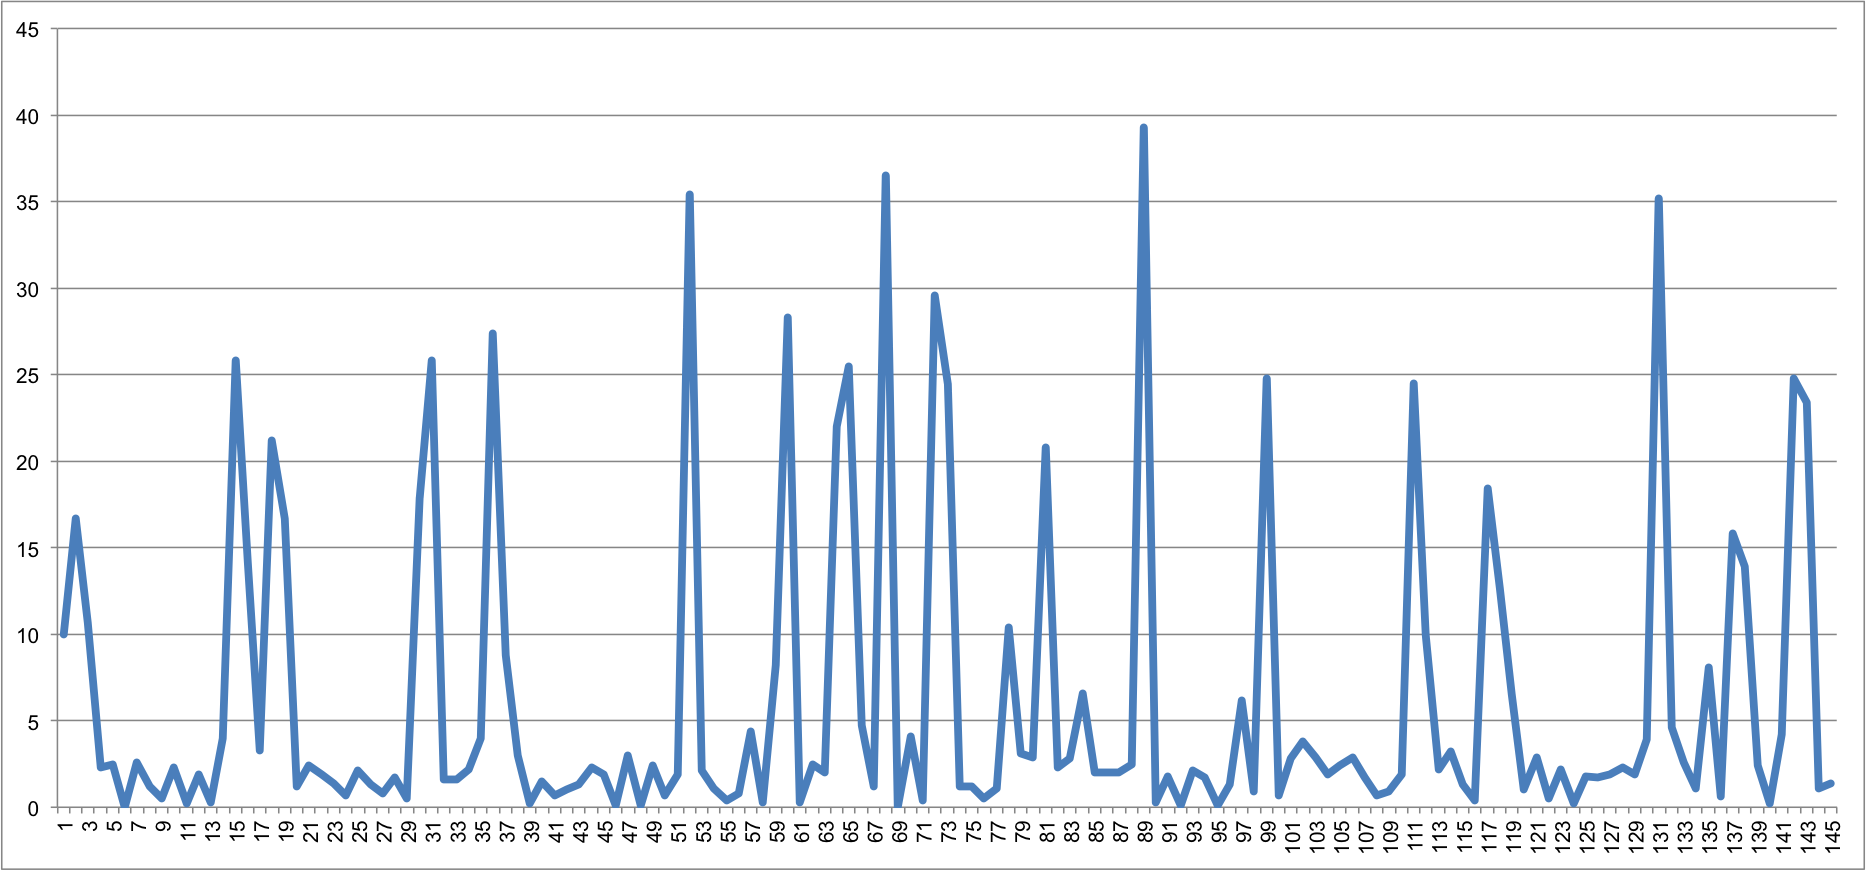
\includegraphics[width=4in]{../northbound.png}  
\caption{\small \sl Northbound Arrival Intervals by Order of Occurrence\label{fig:northbound_arrival}}  
\end{center}  
\end{figure} 

\begin{figure}  
\begin{center}
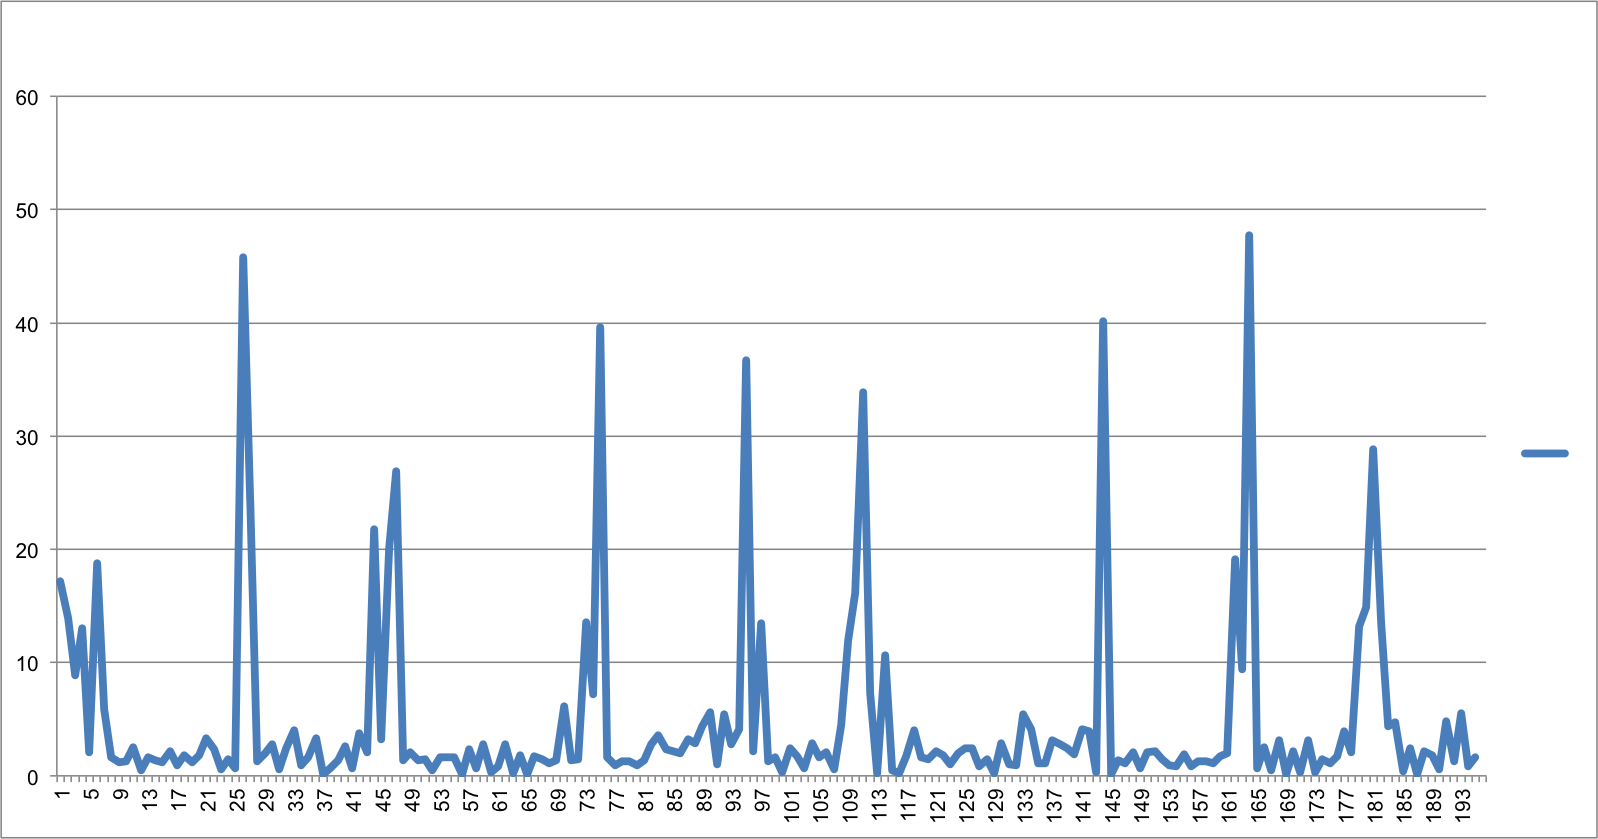
\includegraphics[width=4in]{../southbound.png}
\caption{\small \sl Southbound Arrival Intervals by Order of Occurrence\label{fig:southbound_arrival}}  
\end{center}  
\end{figure} 

The distribution of car arrival is very important, but has been difficult to model. The arrival intervals between 
northbound and southbound cars are provided in \ref{fig:northbound_arrival} and \ref{fig:southbound_arrival}.
Model fitting was attempted for both $\Gamma$ and $\Gamma$-mixture models on the raw data, but resulted in poor
fits. Furthermore, pruning outliers via the common interquartile range approach, where values are rejected when
they lie outside of $median + 1.5IQR$, where $IQR$ is the interquartile range $Q_3 - Q_1$.

Given the difficulties with modelling we'll take a simpler approach and assume the ``true distribution`` is modeled by what was observed,
and simply plan to use the observed frequency distribution as our input distribution. As the project progresses we can
refine this model.

The current light timing of the system is known, and provided in \cite{ngsim}, but we'll allow the user to set
those values dynamically via a UI.

\subsubsection{Data Analysis}
In the \texttt{data\_processing} folder, most of code used for distribution fitting and statistics can be found there.
The data analysis code was written in JavaScript, and runs completely in NodeJS \cite{nodejs}. NPM \cite{npm} was used
to manage dependencies and those dependencies can be seen in the \texttt{package.json} file. Of those packages, I have
authored the \texttt{chi-squared-test} module \cite{chiSquaredNpm}, and the \texttt{gamma-distribution}
\cite{gammaDistributionNpm}. Gulp \cite{gulp} was used a build tool for automating tasks (including building this paper).
To run some of the data analysis code I wrote, you'll need to install and run gulp. Instructions for doing so are
provided in the final section of this paper.

\subsection{Simulation Output}
The most important statistic we'll want to collect during the simulation is the thoughput of the simulation. We'll
want to observe how the light timing affects the average travel time for cars. It will also to see how variable this
is. For instance, do cars travelling on Peachtree St. have similar travel times, despite their arrival time, or does
their arrival drastically lengthen their time to travel the stretch of road we are modeling. 

\subsection{Simplifications and Assumptions}
Probably the most obvious "flaw" in such a design are the simplifications made. Details can certainly be left out
purposely for many reasons such as time constraints, lack of supporting data to model a extra feature, or simply
unneccesary complexity.

In this case, certainly the most prominent would be the ``isolation'' of the model. We are only considering an
idealized random input distribution of cars from both North and South of the 12th St. intersection. However, this is
certainly not the case, since this input distribution is affected by countless other factors like the surrounding
lights, cars passing along 12th at that intersection, and even simply time of day. We assume in this simulation is
perpetually between 4:00PM to 4:15PM in Atlanta (a frightening thought indeed), simply due to the fact that we only
have data for that time range. All in all, we assume the conditions were fairly identical to that in which the 
aforementioned CTS study was made.

Another simplification to consider is lane changing. Lane changing models do exist \cite{lanechanging} \cite{lanechanging2},
but can be complex, requiring modeling of driver choices and gap acceptance for drivers. Peachtree is a two lane road,
so lane changes are possible. However, we will make the assumption that drivers by this point have already made any
discretionary lane changes and traffic is evened out between lanes. Also, we will assume left turning drivers will be
in the left lane already. Similarly, right turning drivers will already be in the right lane.

\section{Simulation Software Architecture}
Because of the event-driven architecture, the system can be though of as a set of event emitters and event listeners.
In some cases, an object may both emit and listen for events.

The first event emitter to consider is the \texttt{CarEmitter}. The \texttt{CarEmitter} uses the measured input
distribution we have for cars and generates a set of cars randomly. It then emits these cars as individual
\texttt{car:arrived} event. There will generally be two \texttt{CarEmitter}s, one for the North and South direction.

The second emitter will be the \texttt{LightSignal}. It will emit \texttt{light:changed} events, passing the light color.
Also, instead of enqueueing these events upfront, it will also listen for \texttt{light:changed} so that its
changing duration can modified on the fly (using the UI).

The \texttt{IntersectionQueue} holds a list of cars lined up at the intersection. It also maintains the
current signal state, so that it can send cars directly through the intersection if the light is green. It responds
to pretty much every event mentioned above. When the light changes, it will need update it's current signal state.
This may mean sending some cars off of the queue and stop holding cars, or to no longer let cars through and make them
wait. Furthermore, when a car arrives it will handle that event by deciding whether the car can pass through or needs
to wait on the light. Also, this class emits events. Whenever a car finally crosses the intersection, it emits
a \texttt{car:exited} event.

Since we want to gather metrics regarding the throughput of cars, we'll also provide a listener class
\texttt{ThroughputStatistics} that will listen for cars to complete their journey through the system. This will
be reported in the UI in real time.

The simulation is written in CoffeeScript \cite{coffeescript}, which is a small language that compiles to JavaScript.
CoffeeScript removes some of the boilerplate associated with setting up prototype chains and other object-oriented
concepts in JavaScript.
Backbone \cite{backbone} along with Underscore \cite{underscore} and jQuery \cite{jquery} were used to provide some
application structure, like basic eventing, and the sorted
collections that are used to form the basis for the event queue and \texttt{IntersectionQueue}. Lastly, Browserify
\cite{browserify} was used to bundle the code into a single file. Minification was done with Uglify.js \cite{uglify}.

\section{Current Build and Running Instructions}
The simulation is currently deployed at \cite{aprilandchip} and currently runs a fixed number of cars through stepping
at 1 second real time being equal to 100ms. Eventually, this will be adjustable in real-time, and better visualized.
Cars are generated regularly at 10 (+ an uniformly random number between 0 and 1) second intervals. Light timings are
currently hard-coded as well. Currently, we're only modeling a single direction, and ignoring turns, and variations
between cars.

To build the application locally, you'll need to install a version of Node.js \cite{nodejs} at 0.10.0 or higher. This will be bundled
with npm. Since this project uses gulp for a task runner, you'll need to install it globally via
\texttt{npm install -g gulp}. Inside the \texttt{simulation} directory, you'll need to pull in packages with just
\texttt{npm install}. Once that installs, running \texttt{gulp} will run the build for you and generate a
\texttt{main.js} that's included in the \texttt{index.html} file. Opening this file in a browser should run the
simulation.

\bibliographystyle{plain}
\bibliography{main}

\end{document}
